\subsection{Actualización de elementos}

  \paragraph{}La figura \ref{capturaActualizacionElementos} muestra un ejemplo
  de actualización de un elemento. Como se puede observar, no se diferencia
  de la interfaz de creación de un nuevo elemento, sino que se obtiene la
  información del elemento para su posterior modificación.


  \begin{figure}[!ht]
    \begin{center}
      \fbox{
        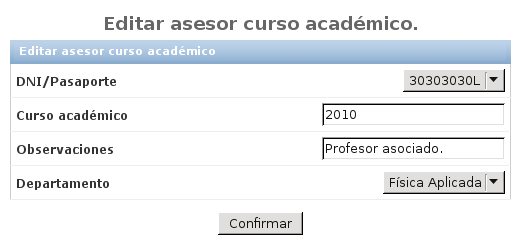
\includegraphics[scale=0.6]{12.Disenyo_Interfaz/12.3.Gestion_Informacion/12.3.3.Actualizacion_Elementos/actualizacion_elementos.png}
      }
      \caption{Captura de pantalla de actualización de un elemento.}
      \label{capturaActualizacionElementos}
    \end{center}
  \end{figure}